\chapter{Experiments}
\label{cha:Experiments}

\section{Evaluation metrics}

\subsection{success\_rate}
The primary metric of evaluation for the developed agents is the $success\_rate$. The $success\_rate$ is defined as the ratio of successful episodes to the total number of episodes. An episode is considered successful if the agent passes through all three goals within the time limit \ref{time_limit}. Collisions of the agent do not disqualify an episode from being succesful, as long as the agent passes all goals.

\subsection{goal\_completion\_rate}

The $goal\_completion\_rate$ is defined as the ratio of passed goals to the total number of goals in the episodes. The $goal\_completion\_rate$ is a more fine-grained metric than the $success\_rate$. However the two metrics are closely related as a high $success\_rate$ implies a high goal\_completion\_rate. The major advantage of the $goal\_completion\_rate$ is that it can used to measure the progress of an agent during training more accurately. 
The $goal\_completion\_rate$ would increase when the agent is able to pass more goals on average, whereas the $success\_rate$ would only increase when the agent is able to pass all goals in an episode more often. The $goal\_completion\_rate$ captures learning progress earlier in training. This behaviour can be observed in training runs, shown in \ref{fig:success_rate_vs_goal_completion_rate}.


\begin{figure}
    \centering
    \subfigure[success\_rate]{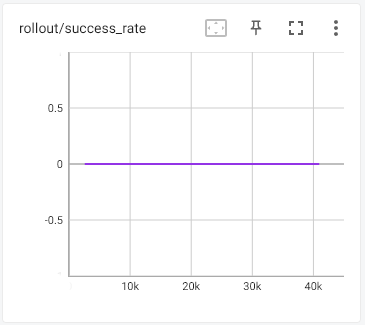
\includegraphics[width=0.3\textwidth]{Bilder/metrics/sr_vs_gcr_success_rate.PNG}}
    \subfigure[goal\_completion\_rate]{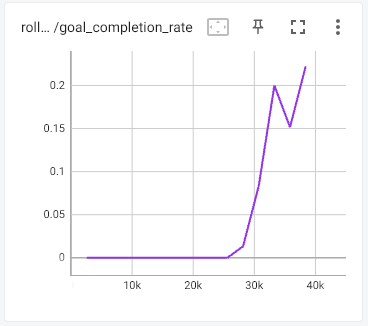
\includegraphics[width=0.3\textwidth]{Bilder/metrics/sr_vs_gcr_goal_completion_rate.PNG}}
    \caption{Difference in success rate and goal completion rate during early stages of training.}
    \label{fig:success_rate_vs_goal_completion_rate}
\end{figure}
% diese Bilder funktionieren nur für frühe Episoden, später sind die Werte sehr gleich


\section{Standard evaluation}






eval() 
the method that runs all the different setups and mainly checks the success\_rate of the model on the different tracks.





\subsection{Deterministic check}

deter or non-deter better

\subsection{identical start condition}

see if the policy is consistent when it is run multiple times with the same start condition



\subsection{Fresh obs vs non-fresh obs}

% ## fresh obs better than nonfresh obs
 
% ### models trained on nonfresh obs

% fresh obs are better than non-fresh obs

% ### models trained on fresh obs

% TODO feasible (time?)


\subsection{policy timestepLength generalization}

policy timestepLength generalization 

what happens to a model trained on fixedTimestepsLength when it is evaluated with a shorter/longer/unrestricted fixedTimestepsLength